\section{Experiments and Results}

\subsection{Dataset}
We used peptide sequences from the Anthem dataset \cite{mei2021anthem}. It consists of 539019, 179673, and 172580 samples for training, validation, and testing, respectively. In more detail, in Fig. S1, we present the distribution of samples by k-mers; 9-mers comprise the majority of samples in the database.

\subsection{Binary classifier and metrics}
The pMHC binding prediction problem is a regression problem. Nonetheless, based on the dataset employed in this study, it could also be approached as a binary classification problem by selecting an appropriate threshold. Moreover, the machine learning metrics used in this work are: Accuracy (Acc.), Precision (Precis.), Recall, F1-score (F1-sc), and Area Under the Curve (AUC).

\subsection{The layer freezing methodology}

For the layer freezing methodology, we froze all Transformer's parameters and just trained the BiLSTM block. Using this method speeds up the training and still achieves good performance, as discussed in prior works \cite{merchant2020happens,lee2019would,kovaleva2019revealing}.

The performance comparison is presented in Table \ref{tab:comparison_3_epochs}; moreover, Fig. \ref{fig:comparison_3_3pochs} shows the AUC of each model using GAS, and the layer freezing methodology. In this comparison, the suffix 'Normal' stands for custom training using all hyperparameters of Section \ref{sec:fine-tuned}; the suffix 'GAS' signifies the integration of Gradient Accumulation Steps (GAS), while the suffix 'Freeze' is indicative of our application of the layer freezing methodology to the models. Based on the obtained results, it is evident that the implementation of the layer freezing methodology leads to performance enhancements across all ESM2 models. Additionally, it was observed that the larger models, such as ESM2(t30)-Normal, ESM2(t33)-Normal, TAPE-Normal, and ProtBert-Normal, failed to converge due to a gradient vanishing problem, which will be elaborated upon in the subsequent section. Furthermore, the utilization of the layer freezing methodology enables these models to converge effectively.

\begin{figure}[h]
	\centering
	
	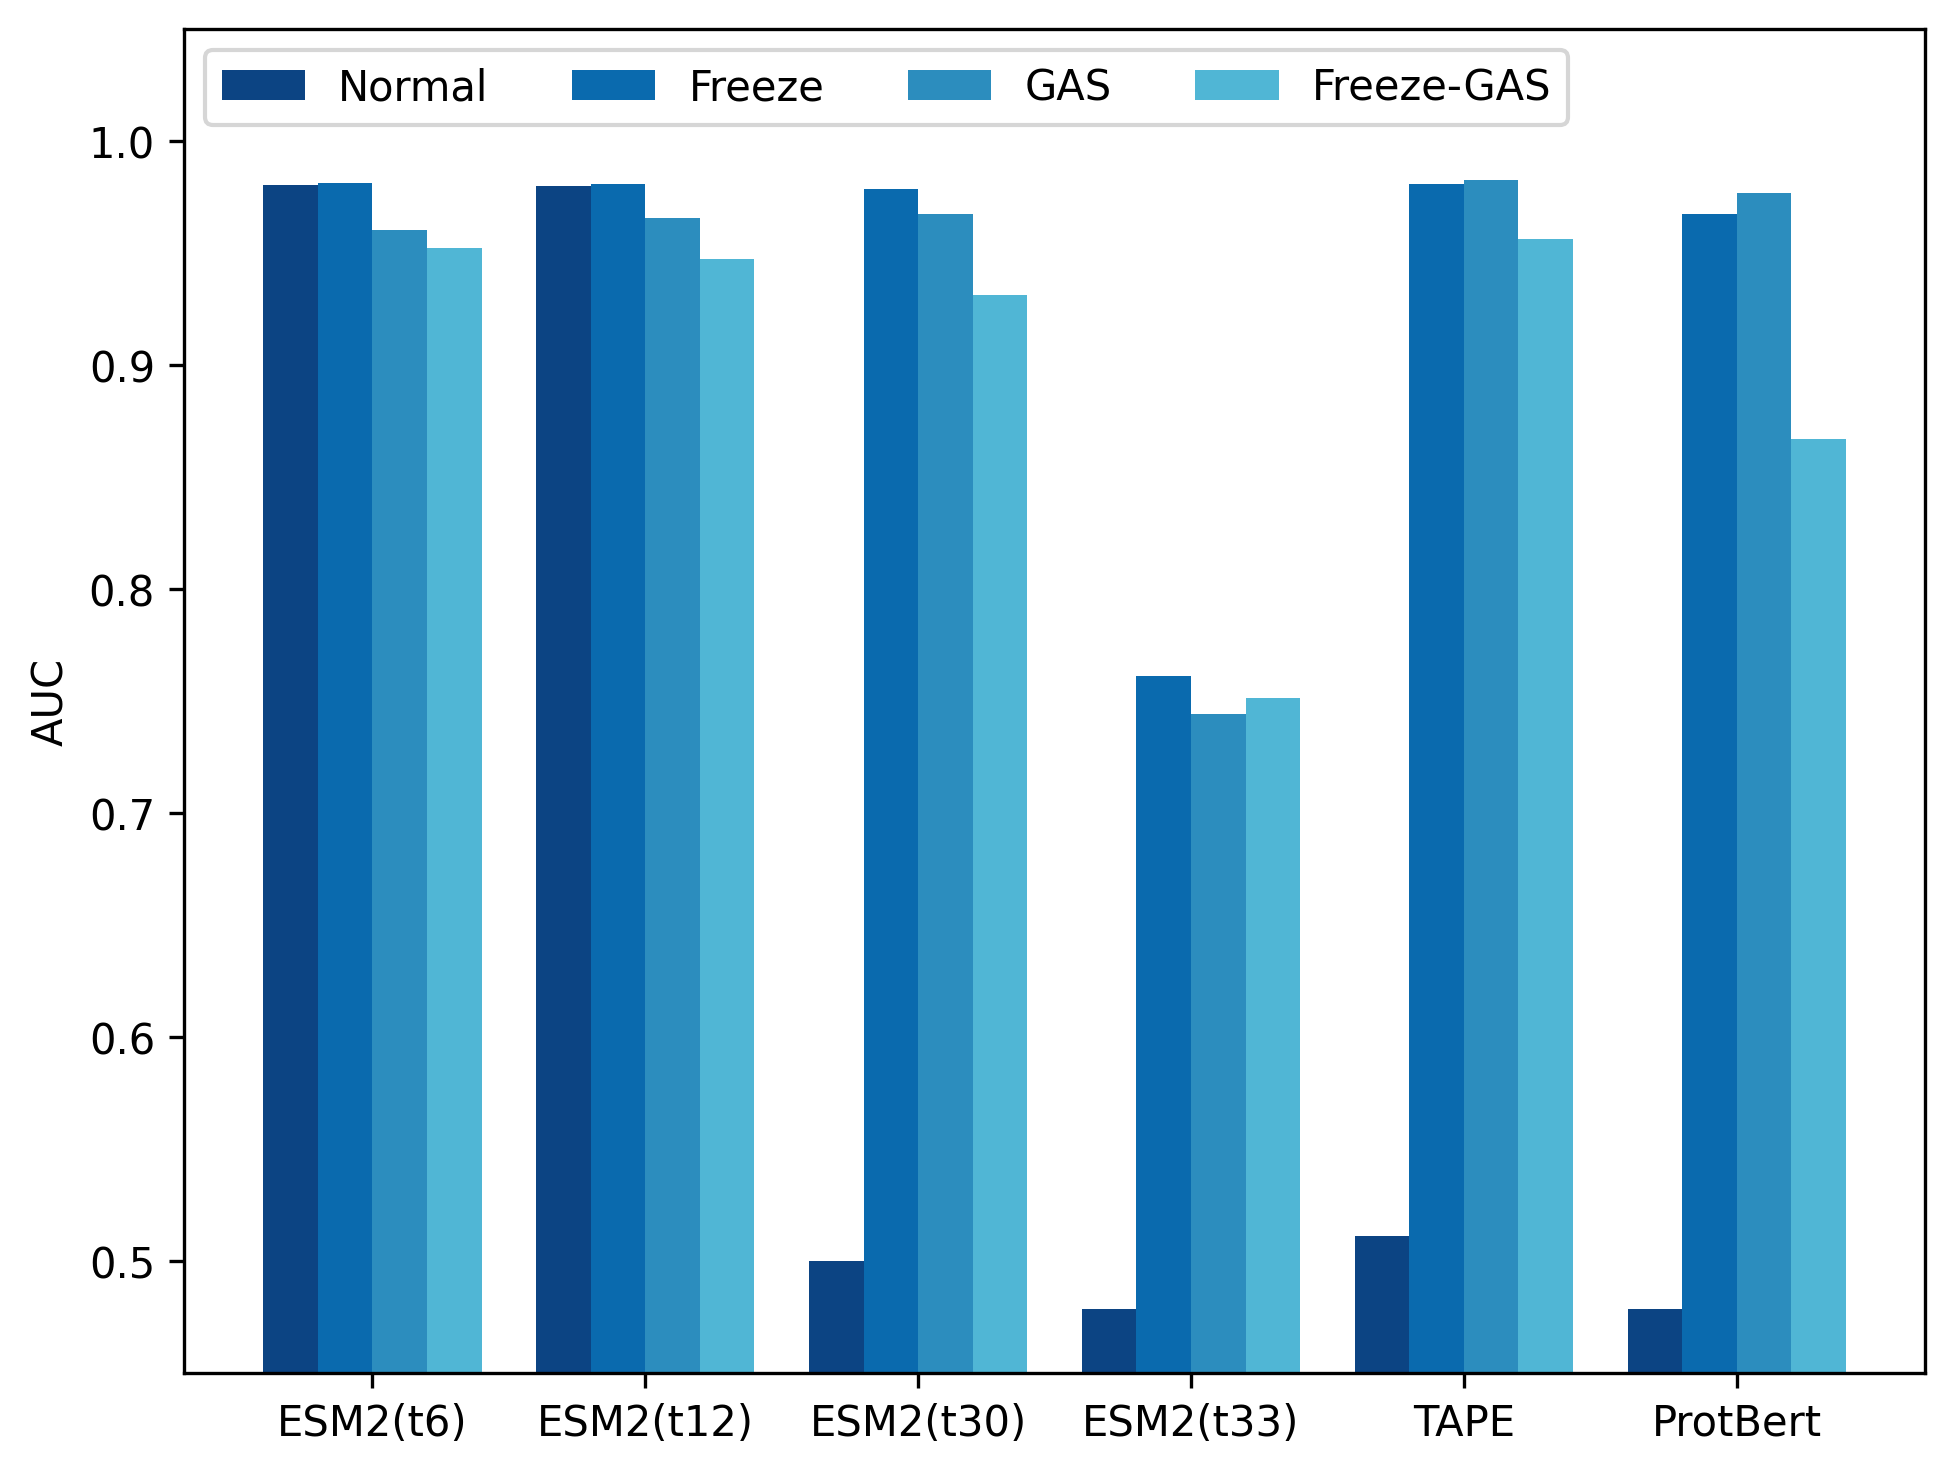
\includegraphics[width=0.42\textwidth]{../img/results/metrics_comparion_by_model}	
	
	\caption{Comparative analysis of Area Under the Curve (AUC) in Transformer model architectures using various training methodologies, including standard training (Normal), training with a layer freezing methodology (Freeze), training with Gradient Accumulation Steps (GAS), and training Combining GAS with layer freezing (Freeze-GAS). Moreover, we trained all models for three epochs.}
	\label{fig:comparison_3_3pochs}
\end{figure}



\begin{table}[h]
	\centering
	\caption{Performance evaluation of Transformer models with Gradient Accumulation Steps (GAS) and the layer freezing methodology \textbf{trained for three epochs}. Moreover, the suffix 'Normal' stands for classic training using hyperparameters of Section \ref{sec:fine-tuned}. The inclusion of the suffix 'GAS' in each model signifies the integration of Gradient Accumulation Steps, while the suffix 'Freeze' is indicative of our application of the layer freezing methodology to the models. Furthermore, the '-' in each cell signifies that the model could not converge.}
	\label{tab:comparison_3_epochs}
	
	\tiny
	\begin{tabular}{llllll} \hline
		\textbf{Model}       & \textbf{Acc.} & \textbf{Precis.} & \textbf{Recall} & \textbf{F1-sc.} & \textbf{AUC}   % & \textbf{MCC}    
		\\ \hline
		ESM2(t6)-Normal             & 0.9344            & \textbf{0.9334}    & 0.9354          & 0.9344            & 0.9805          %& 0.8689          
		\\
		ESM2(t6)-Freeze      & \textbf{0.9351}   & 0.9253             & \textbf{0.9464} & \textbf{0.9357}   & \textbf{0.9812} %& \textbf{0.8704} 
		\\
		ESM2(t6)-GAS         & 0.8986            & 0.8966             & 0.9007          & 0.8986            & 0.9602          %& 0.7973          
		\\
		ESM2(t6)-Freeze-GAS  & 0.8869            & 0.8913             & 0.8806          & 0.8860            & 0.9520          %& 0.7738          
		\\ \hline
		
		
		ESM2(t12)-Normal            & 0.9327            & 0.9243             & 0.9422          & 0.9332            & 0.9799          %& 0.8655          
		\\
		ESM2(t12)-Freeze     & \textbf{0.9344}   & \textbf{0.9251}    & \textbf{0.9451} & \textbf{0.9350}   & \textbf{0.9808} %& \textbf{0.8690} 
		\\
		ESM2(t12)-GAS        & 0.9010            & 0.9279             & 0.8692          & 0.8976            & 0.9655          %& 0.8037          
		\\
		ESM2(t12)-Freeze-GAS & 0.8805            & 0.8556             & 0.9149          & 0.8843            & 0.9475          %& 0.7629          
		\\ \hline
		
		
		ESM2(t30)-Normal            & -                 & -                  & -               & -                 & -               %& -               
		\\
		ESM2(t30)-Freeze     & \textbf{0.9303}   & \textbf{0.9185}    & \textbf{0.9440} & \textbf{0.9311}   & \textbf{0.9786} %& \textbf{0.8609} 
		\\
		ESM2(t30)-GAS        & 0.9090            & 0.9167             & 0.8993          & 0.9079            & 0.9675          %& 0.8181          
		\\
		ESM2(t30)-Freeze-GAS & 0.8565            & 0.8156             & 0.9206          & 0.8649            & 0.9312          %& 0.7191          
		\\ \hline
		
		
		ESM2(t33)-Normal            & -                 & -                  & -               & -                 & -               %& -               
		\\
		ESM2(t33)-Freeze     & \textbf{0.6818}   & \textbf{0.7139}    & 0.6044          & 0.6546            & \textbf{0.7613} %& 0.3677          
		\\
		ESM2(t33)-GAS        & 0.6767            & 0.6312             & 0.8467          & 0.7233            & 0.7442         % & \textbf{0.3763} 
		\\
		ESM2(t33)-Freeze-GAS & 0.6738            & 0.6254             & \textbf{0.8633} & \textbf{0.7254}   & 0.7514          %& 0.3763          
		\\ \hline
		
		
		TAPE-Normal                 & -                 & -                  & -               & -                 & -               %& -               
		\\
		TAPE-Freeze          & 0.9342            & 0.9276             & 0.9415          & 0.9345            & 0.9809          %& 0.8684          
		\\
		TAPE-GAS             & \textbf{0.9371}   & \textbf{0.9290}    & \textbf{0.9463} & \textbf{0.9376}   & \textbf{0.9826} %& \textbf{0.8744} 
		\\
		TAPE-Freeze-GAS      & 0.8914            & 0.8851             & 0.8989          & 0.8920            & 0.9564          %& 0.7828          
		\\ \hline
		
		
		ProtBert-Normal             & -                 & -                  & -               & -                 & -               %& -               
		\\
		ProtBert-Freeze      & 0.9083            & 0.9176             & 0.8968          & 0.9071            & 0.9673          %& 0.8168          
		\\
		ProtBert-GAS         & \textbf{0.9138}   & \textbf{0.9569}    & 0.8662          & \textbf{0.9093}   & \textbf{0.9767} %& \textbf{0.8313} 
		\\
		ProtBert-Freeze-GAS  & 0.7864            & 0.7333             & \textbf{0.8988} & 0.8076            & 0.8669          %& 0.5881         
		\\ \hline
	\end{tabular}
\end{table}





\subsection{Vanish gradient and GAS}

In Table \ref{tab:comparison_3_epochs}, we noticed that large models like ESM2(t30)-Normal, ESM2(t33)-Normal, TAPE-Normal, and ProtBert-Normal didn't converge. Thus, we plotted the gradients of these models during training in order to discover their causes. First, we plotted mean gradients by layer for the smallest model ESM2(t6)-Normal in Fig. S2 (this model didn't vanish gradients). Then, we plotted mean gradients for ESM2(t30)-Normal (this model got into vanish gradient problem) in Fig. S3. As evident from the results, the larger model ESM2(t30) exhibited almost zero mean gradients across all Bert layers after just three epochs; consequently, this phenomenon rendered the model unable to converge effectively.


Gradient Accumulation Steps (GAS) is usually used to reduce GPU memory storage problem during training \cite{zhang2023adam,huang2023measuring}. Moreover, it could slightly alleviate the vanish gradient problem by accumulating gradients over some batches and only stepping the optimizer after a number of batches have been performed. For instance, in Table \ref{tab:comparison_3_epochs}, we show the results after applying GAS to all Transformer models after training for three epochs. For instance, the models ESM2(t30)-Normal, ESM2(t33)-Normal, TAPE-Normal, and ProtBert-Normal without GAS didn't converge; however, if we trained them with GAS, they reached acceptable results. 



In particular, the incorporation of Gradient Accumulation Steps (GAS) in TAPE-GAS not only mitigates the gradient vanishing issue but also enhances performance when compared to other experiments involving TAPE, such as TAPE-Normal, TAPE-Freeze, and TAPE-Freeze-GAS. The same phenomenon was observed in the ProtBert models as well.





\subsection{Training for 30 epochs}

For a more detailed comparison, we extended the training epochs of the best-performing models from Table \ref{tab:comparison_3_epochs}, including ESM2(T6) and TAPE, to 30 epochs with early stopping. Additionally, we included ESM2(t30) to investigate whether larger models achieve improved results over a longer training period. It is worth noting that ProtBert-BFD was excluded from the analysis due to its poor performance. As indicated in Table \ref{tab:comparison}, the ESM2 models yield their best results when the layer freezing methodology is applied. In contrast, for TAPE, the best results are achieved when using GAS without freezing. Notably, TAPE-GAS and ESM2(t6)-Freeze produced the most favorable outcomes, with TAPE-GAS slightly outperforming ESM2(t6)-Freeze in this regard.




\begin{table}[]
	\centering
	\caption{Performance evaluation of Transformer models with Gradient Accumulation Steps (GAS) and the layer freezing methodology \textbf{trained for thirty (30) epochs}. Moreover, the suffix 'Normal' stands for classic training using hyperparameters of Section \ref{sec:fine-tuned}. The inclusion of the suffix 'GAS' in each model signifies the integration of Gradient Accumulation Steps, while the suffix 'Freeze' is indicative of our application of the layer freezing methodology to the models. Furthermore, the '-' in each cell signifies that the model could not converge.}
	\label{tab:comparison}
	\tiny
	\begin{tabular}{llllll} \hline
		\textbf{}            & \textbf{Acc.} & \textbf{Precis.} & \textbf{Recall} & \textbf{F1-sc.} & \textbf{AUC}      \\ \hline
		ESM2(t6)-Normal             & 0.9390            & 0.9333             & \textbf{0.9453} & 0.9392            & 0.9797                    \\
		
		ESM2(t6)-Freeze      & \textbf{0.9401}   & \textbf{0.9398}    & 0.9402          & \textbf{0.9400}   & \textbf{0.9830}          \\
		ESM2(t6)-GAS         & 0.9366            & 0.9322             & 0.9413          & 0.9368            & 0.9818                           \\
		ESM2(t6)-Freeze-GAS  & 0.9354            & 0.9326             & 0.9383          & 0.9355            & 0.9813                             \\ \hline
		ESM2(t30)-Normal            & -                 & -                  & -               & -                 & -                                    \\
		ESM2(t30)-Freeze     & \textbf{0.9393}   & 0.9304             & \textbf{0.9493} & \textbf{0.9397}   & 0.9787                      \\
		ESM2(t30)-GAS        & 0.9346            & \textbf{0.9337}    & 0.9352          & 0.9345            & 0.9808                            \\
		ESM2(t30)-Freeze-GAS & 0.9363            & 0.9319             & 0.9411          & 0.9365            & \textbf{0.9818}                     \\ \hline
		TAPE-Normal                 & -                 & -                  & -               & -                 & -                              \\
		TAPE-Freeze          & 0.9395            & \textbf{0.9404}    & 0.9382          & 0.9393            & 0.9815                           \\
		TAPE-GAS             & \textbf{0.9415}   & 0.9352             & \textbf{0.9484} & \textbf{0.9418}   & \textbf{0.9841}            \\
		TAPE-Freeze-GAS      & 0.9359            & 0.9297             & 0.9428          & 0.9362            & 0.9820                    \\ \hline    
	\end{tabular}
\end{table}


\subsection{Comparison with state-of-art methods}
Additionally, we compare the best models: ESM2(t6)-Freeze and TAPE-GAS trained for 30 epochs (see Table \ref{tab:comparison}) with state-of-art methods. We covered NetMHCpan4.1 \cite{reynisson2020netmhcpan}, and MHCFlurry2.0 \cite{o2020mhcflurry} because are well-know baselines methods; and three latest tools such as Anthem \cite{mei2021anthem},  Acme \cite{hu2019acme} and MixMHCpred2.2  \cite{gfeller2023improved}. 
During our evaluation of these tools on the test dataset, we encountered specific considerations for ACME. To ensure a fair assessment, we excluded the following alleles from the evaluation for ACME: HLA-C01:02, HLA-C02:02, HLA-C03:03, HLA-C03:04, HLA-C04:01, HLA-C05:01, HLA-C06:02, HLA-C07:01, HLA-C07:02, HLA-C07:04, HLA-C08:02, HLA-C12:03, HLA-C14:02, HLA-C15:02, HLA-C16:01, HLA-C17:01, HLA-A02:50, HLA-A24:06, HLA-A24:13, HLA-A32:15, HLA-B45:06, and HLA-B83:01. This exclusion was necessary as ACME was unable to predict peptide-MHC binding for these particular alleles,

It's worth noting that the choice of threshold for predicting pMHC binding can vary depending on the specific tool and k-mer used. This variability makes the AUC an ideal metric for comparing methods, as it provides a robust evaluation that isn't sensitive to threshold differences. For that reason, in  Figure \ref{fig:comparison_final} and \ref{fig:ROC_comparison_final}, we present the AUC and ROC curve respectively of TAPE-GAS, ESM2(t6)-Freeze, NetMHCpan4.1, and MHCFlurry2.0, Anthem,  Acme, and MixMHCpred2.2. According to these plots, TAPE-GAS, ESM2(t6)-Freeze got the highest AUC value.

Furthermore, when assessing binary classification performance metrics, we standardized the threshold for TAPE-GAS and ESM2(t6) at 0.5. We maintained a threshold of 0.5 for NetMHCpan4.1, in accordance with its recommended setting, while for ACME, we adhered to a threshold of 0.42, as advised in its documentation. In the case of Anthem, the tool provided binary binding predictions directly. However, for MixMHCpred2.2 and MHCfurry, we determined the optimal threshold values from the test dataset, resulting in 2.7308 and 0.09439, respectively. In Table \ref{tab:final_comparison}, we present a comprehensive comparison between TAPE-GAS and ESM2(t6)-Freeze (trained for 30 epochs), and state-of-the-art methods. The results clearly demonstrate that TAPE-GAS and ESM2(t6)-Freeze consistently outperform the existing state-of-the-art tools across all these metrics: AUC, Accuracy, Recall, F1-score, and MCC. 

\begin{figure}
	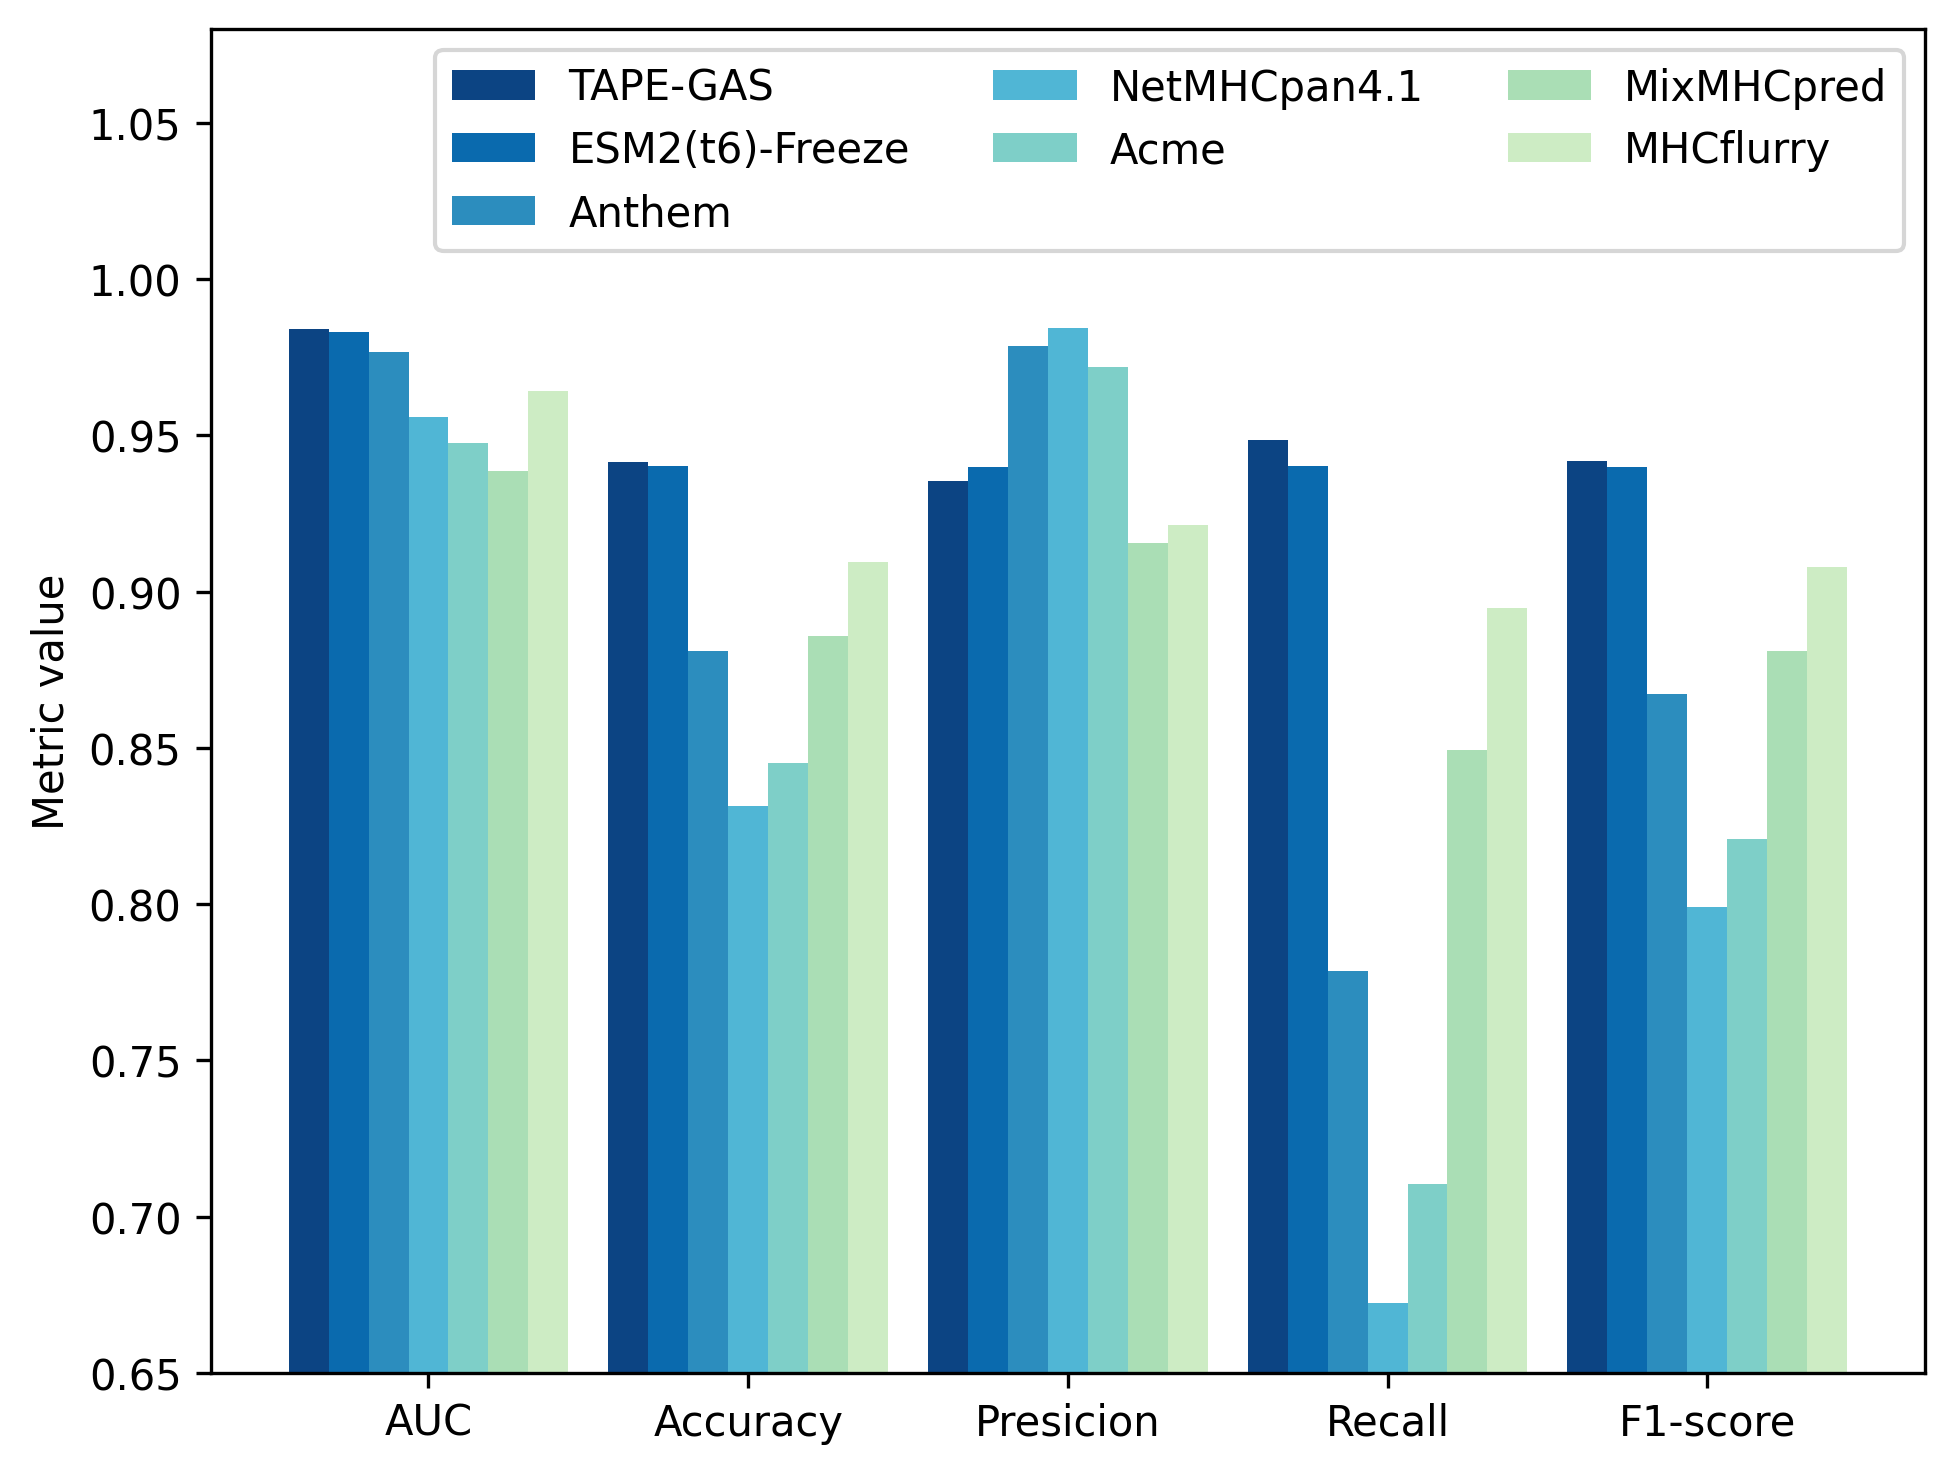
\includegraphics[width=0.45\textwidth]{../img/results/metrics_comparison}
	\caption{The AUC values for TAPE-GAS and ESM2(t6) trained for 30 epochs, in comparison to state-of-the-art methods.}
	\label{fig:comparison_final}
\end{figure}

\begin{figure}
	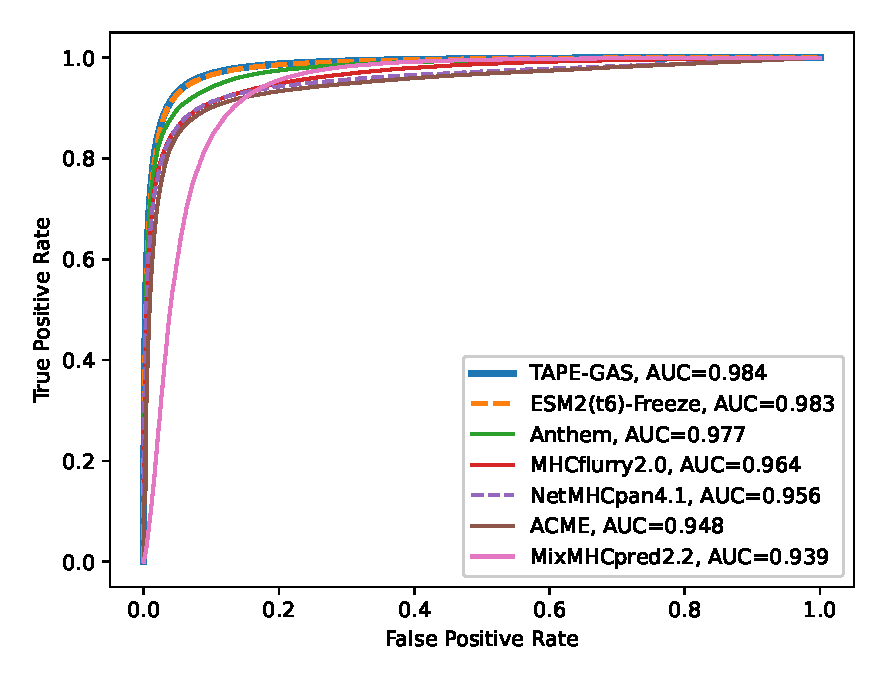
\includegraphics[width=0.45\textwidth]{../img/results/ROC_comparison}
	\caption{ROC curves for TAPE-GAS and ESM2(t6) trained for 30 epochs, in comparison to state-of-the-art methods.}
	\label{fig:ROC_comparison_final}
\end{figure}


\begin{table}[]
	\centering
	\caption{Performance evaluation of Transformer models TAPE-GAS and ESM2(t6)-Freeze, trained for 30 epochs, against Anthem, NetMHCpan4.1, ACME, MixMHCpred2.2, and MhcFlurry2.0.}
	\label{tab:final_comparison}
	\tiny
	\begin{tabular}{lllllll} \hline
		& \textbf{Acc.} & \textbf{Precis.} & \textbf{Recall} & \textbf{F1-sc} & \textbf{AUC}    & \textbf{MCC}    \\ \hline
		TAPE-GAS        & \textbf{0.9415}   & 0.9352             & \textbf{0.9484} & \textbf{0.9418}   & \textbf{0.9841} & \textbf{0.8831} \\
		ESM2(t6)-Freeze & \textbf{0.9401}   & 0.9398             & \textbf{0.9402} & \textbf{0.9400}   & \textbf{0.9830} & \textbf{0.8802} \\
		
		Anthem          & 0.8811            & \textbf{0.9786}    & 0.7787          & 0.8673            & 0.9768          & 0.7785          \\
		NetMHCpan4.1    & 0.8312            & \textbf{0.9844}    & 0.6724          & 0.7991            & 0.9557          & 0.6982          \\
		
		ACME            & 0.8452            & 0.9717             & 0.7105          & 0.8208            & 0.9476          & 0.7165          \\
		MixMHCpred2.2   & 0.8857            & 0.9155             & 0.8493          & 0.8811            & 0.9386          & 0.7733          \\
		MhcFlurry2.0    & 0.9093            & 0.9211             & 0.8948          & 0.9078            & 0.9642          & 0.8189 \\ \hline        
	\end{tabular}
\end{table}


Finally, we show the AUC distribution for TAPE-GAS and ESM2(t6)-Freeze, both trained for 30 epochs, along with Anthem, NetMHCpan4.1, ACME, MixMHCpred2.2, and MHCflurry2.0. In this case, we evaluated each distribution by k-mer (Fig. \ref{fig:auc_distribution}). In all k-mer, TAPE-GAS and ESM2(t6)-Freeze present the highest score. Furthermore, it's worth noting that the compact ESM2(t6)-Freeze model delivers superior results for longer peptides with lengths of 11, 12, 13, and 14.


\begin{figure*}[h]
	\centering
	%\begin{subfigure}[b]{0.3\textwidth}
	%	\centering
	%	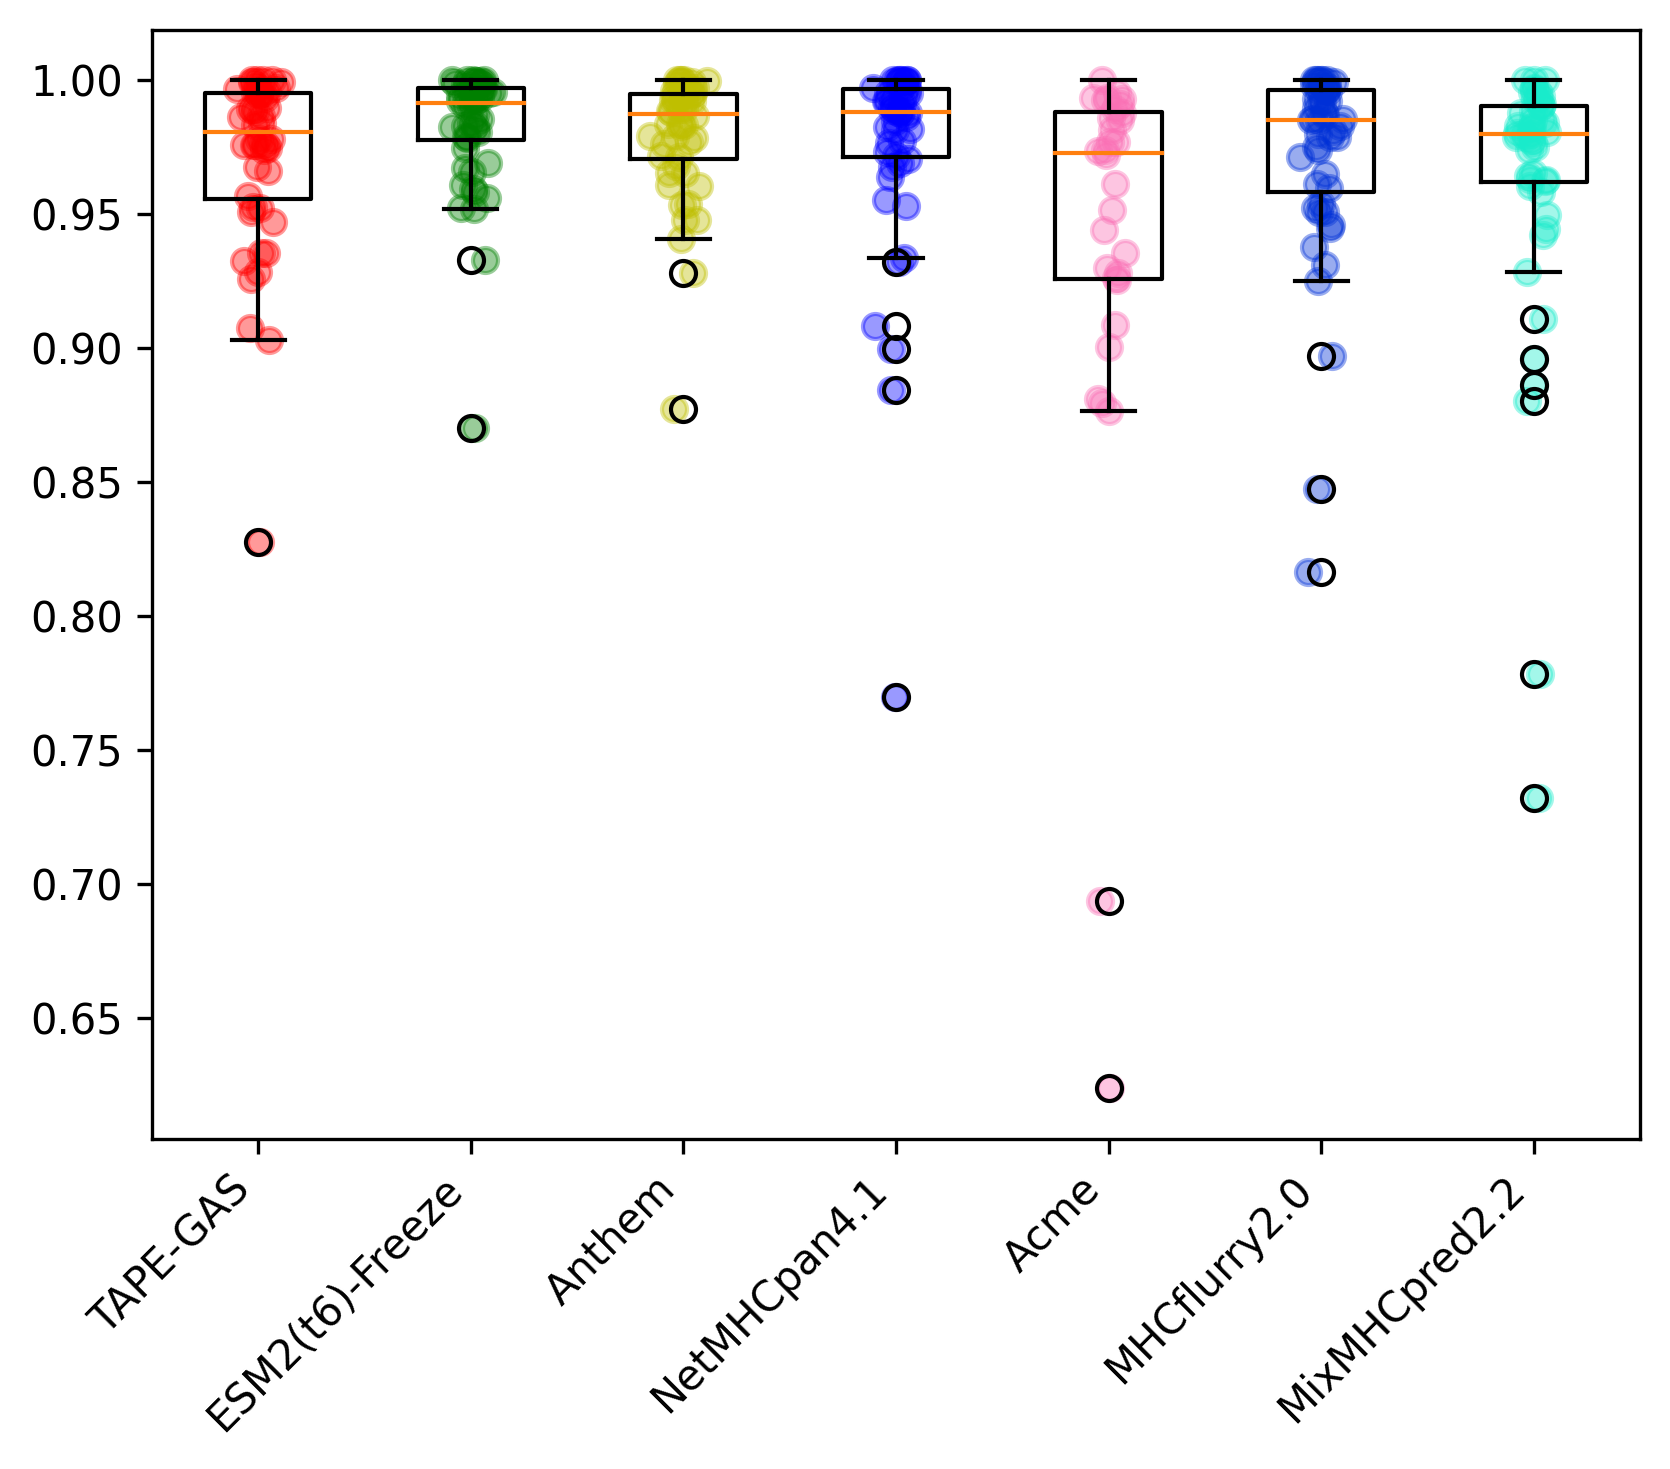
\includegraphics[width=\textwidth]{img/results/auc_distribution_8-mer.eps}
	%	\caption{8-mer}
	%	\label{fig:comparison_8}
	%\end{subfigure}
	%\hfill
	\begin{subfigure}[b]{0.3\textwidth}
		\centering
		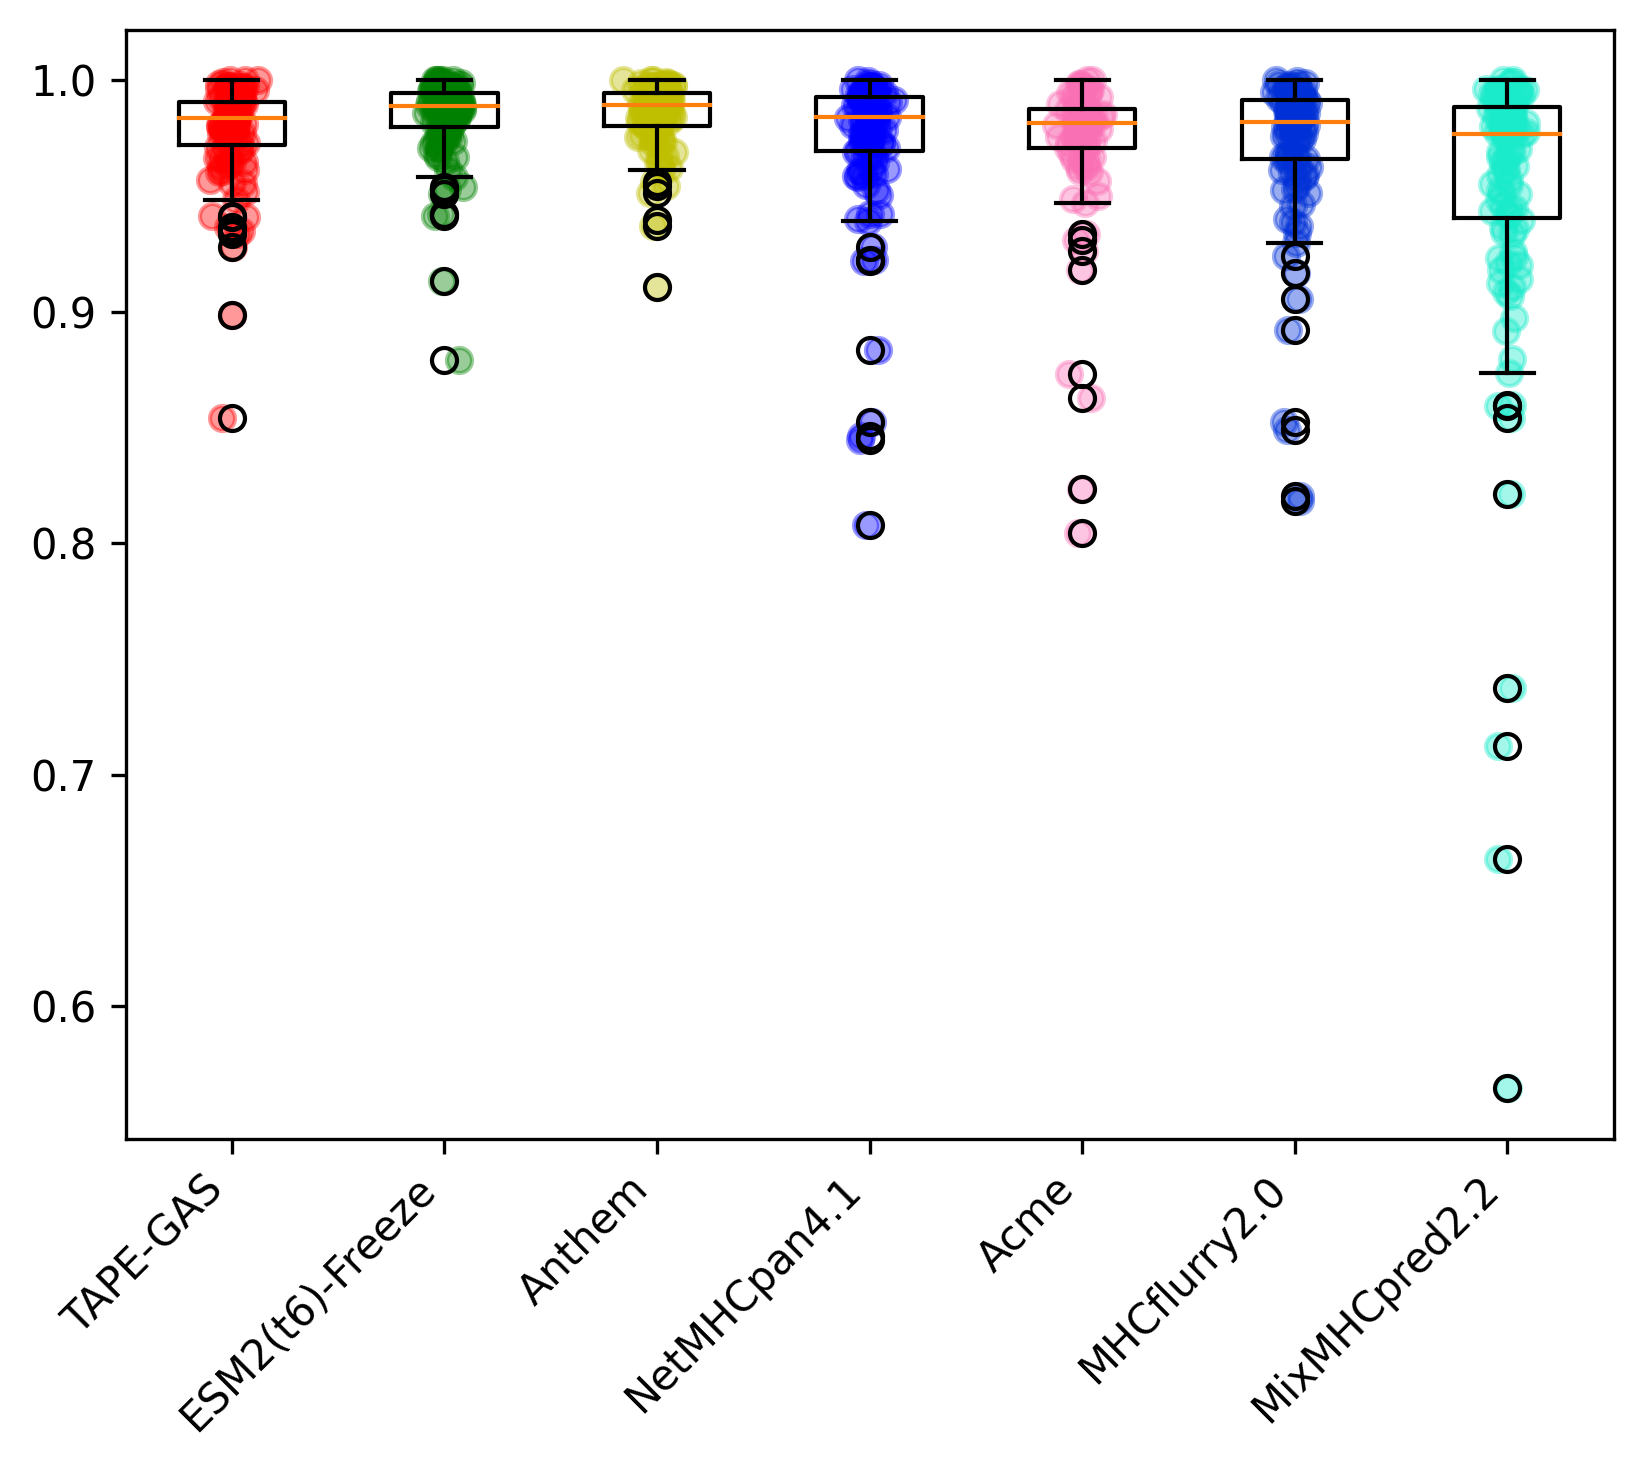
\includegraphics[width=\textwidth]{../img/results/auc_distribution_9-mer}
		\caption{9-mer}
		\label{fig:comparison_9}
	\end{subfigure}
	\hfill
	\begin{subfigure}[b]{0.3\textwidth}
		\centering
		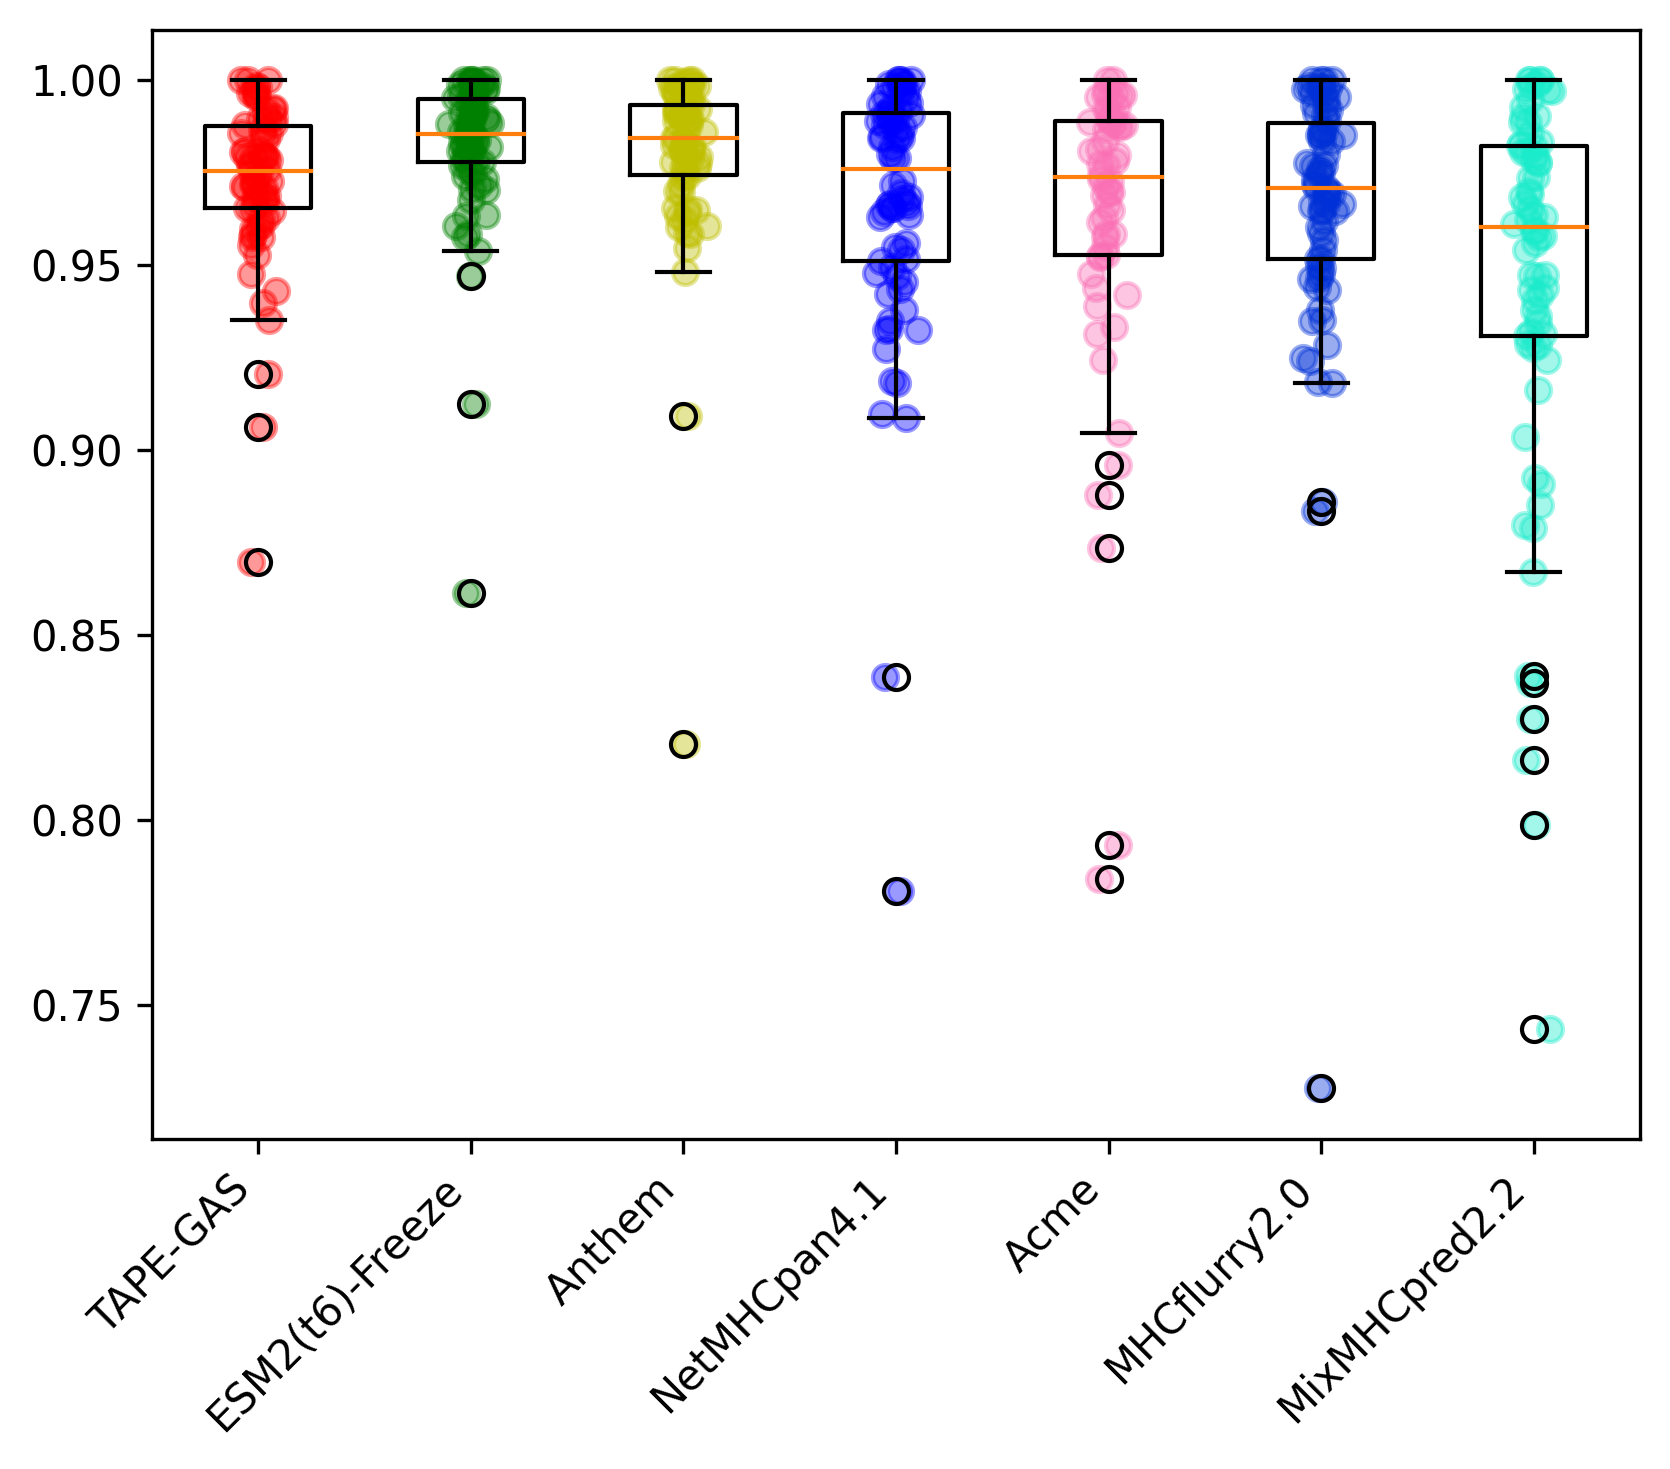
\includegraphics[width=\textwidth]{../img/results/auc_distribution_10-mer}
		\caption{10-mer}
		\label{fig:comparison_10}
	\end{subfigure}
	\hfill
	\begin{subfigure}[b]{0.3\textwidth}
		\centering
		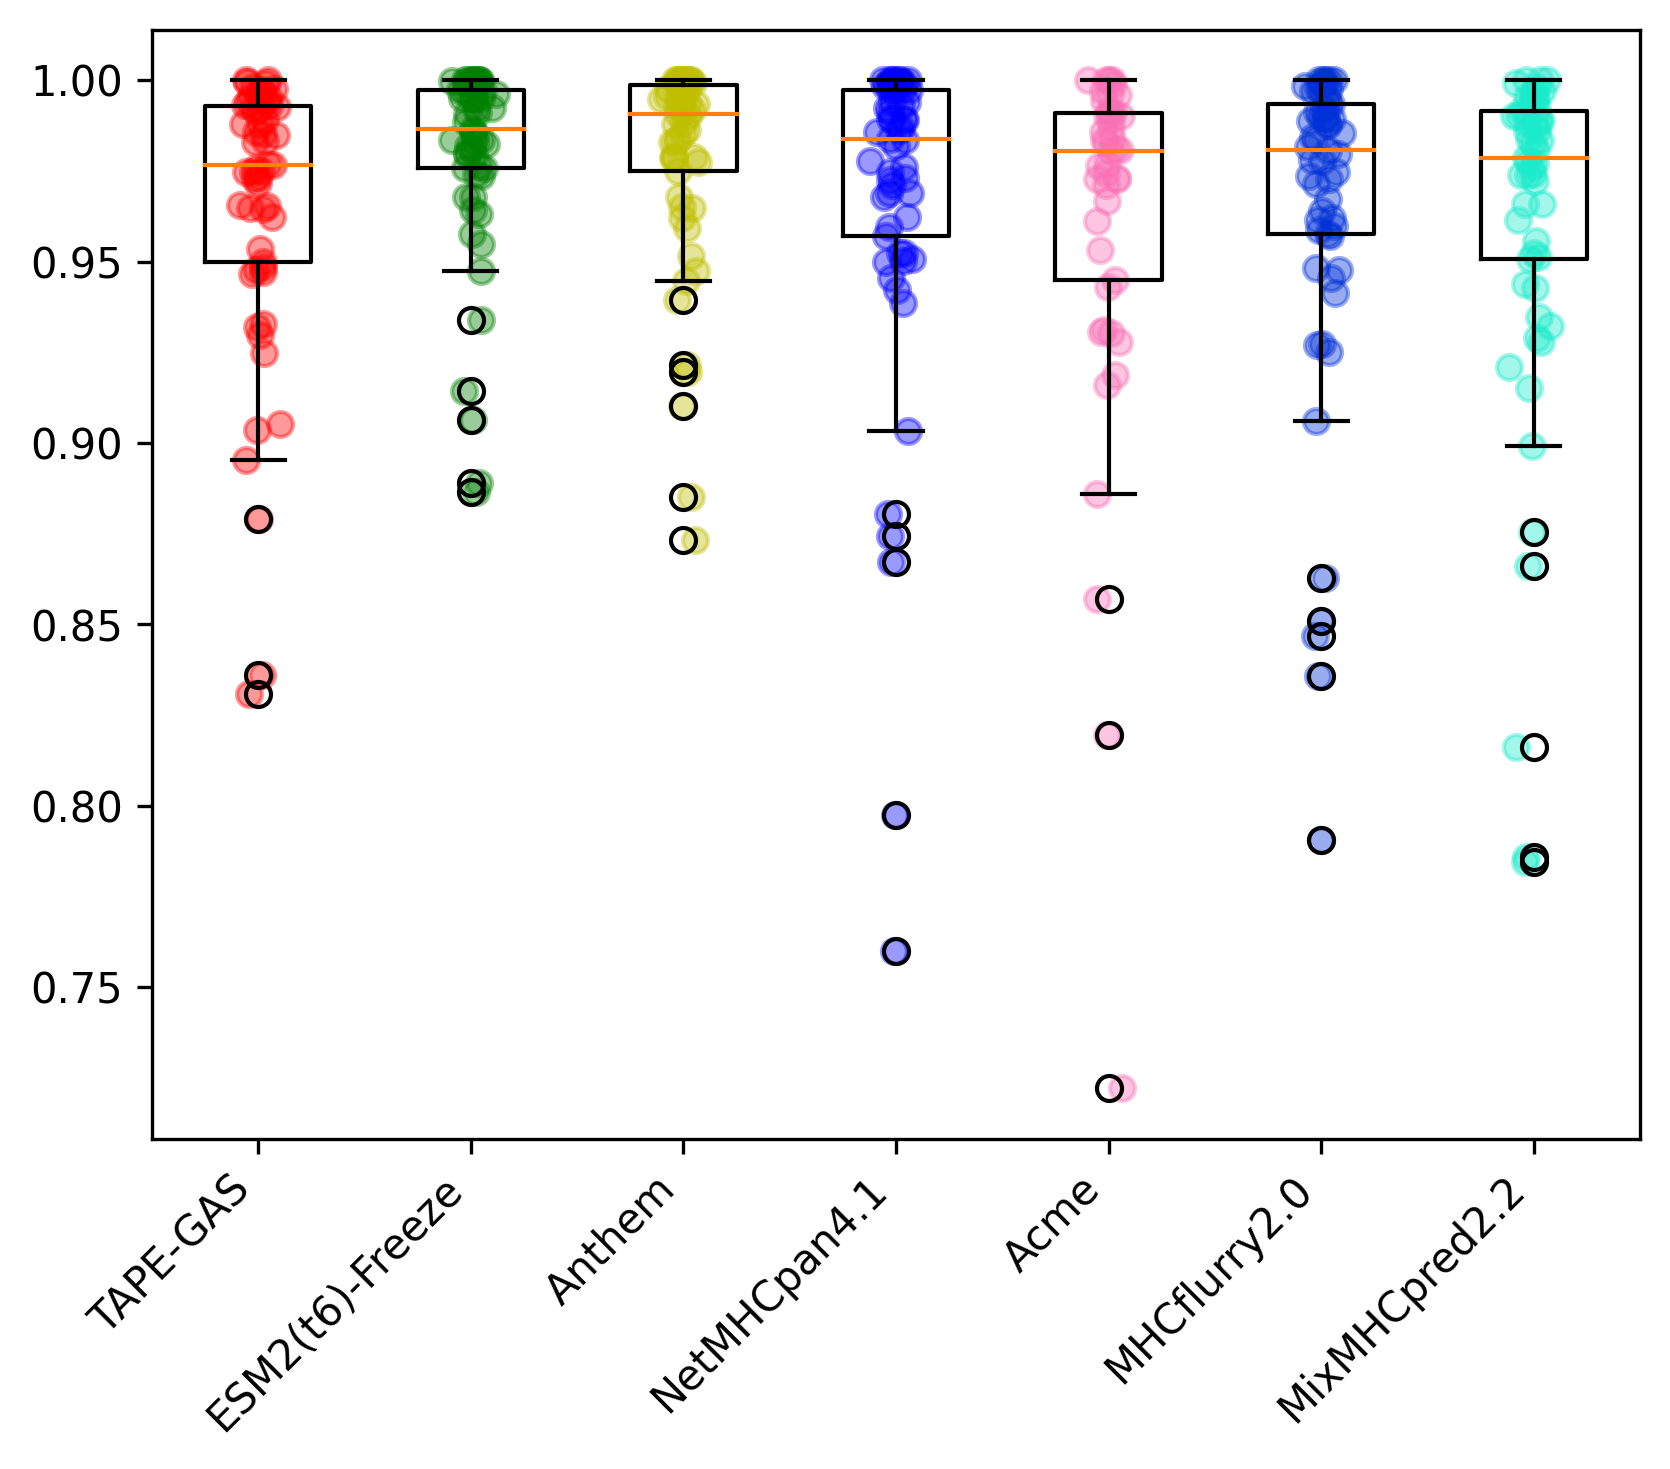
\includegraphics[width=\textwidth]{../img/results/auc_distribution_11-mer}
		\caption{11-mer}
		\label{fig:comparison_11}
	\end{subfigure}
	\hfill
	\begin{subfigure}[b]{0.3\textwidth}
		\centering
		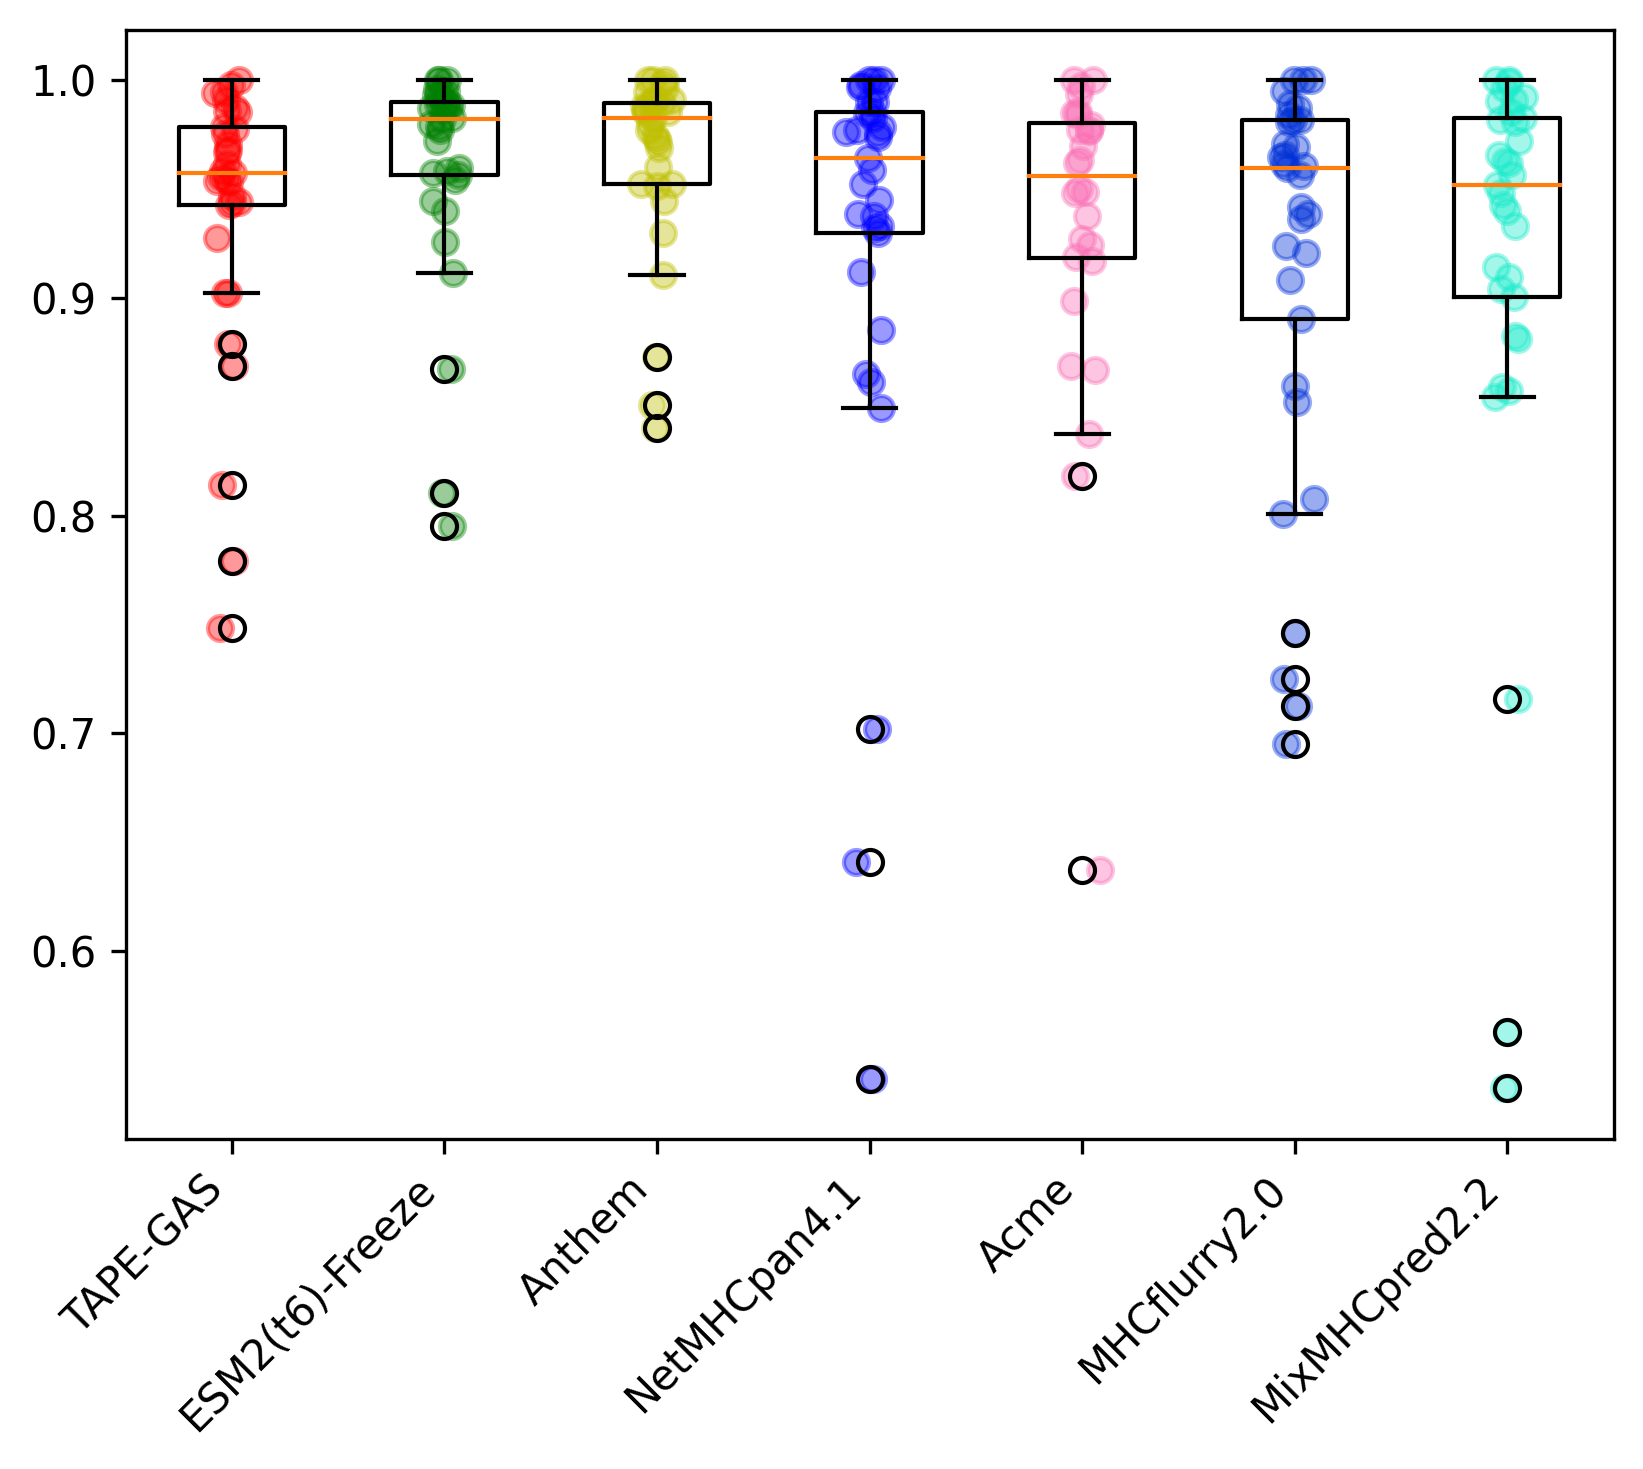
\includegraphics[width=\textwidth]{../img/results/auc_distribution_12-mer}
		\caption{12-mer}
		\label{fig:comparison_12}
	\end{subfigure}
	\hfill
	\begin{subfigure}[b]{0.3\textwidth}
		\centering
		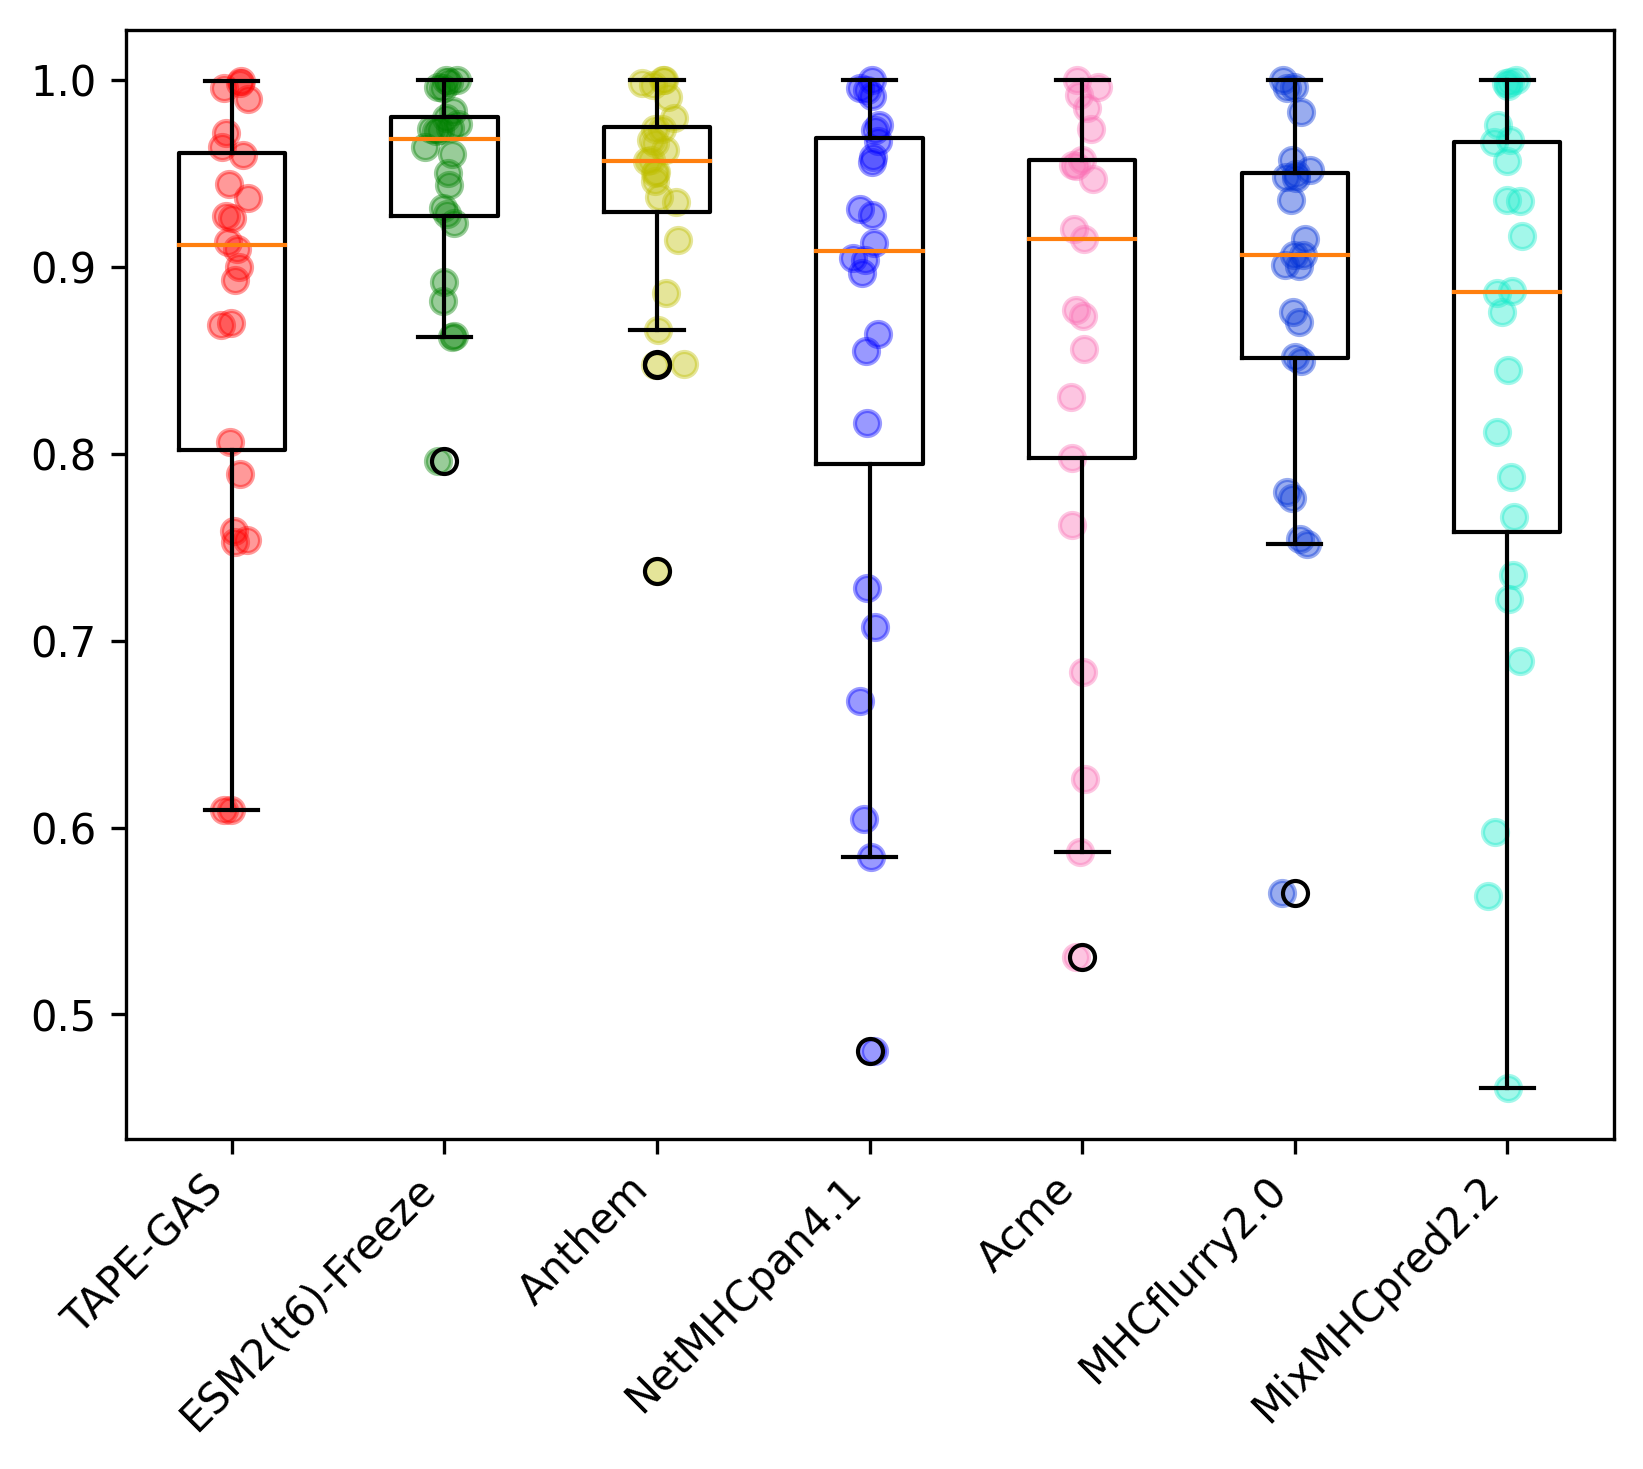
\includegraphics[width=\textwidth]{../img/results/auc_distribution_13-mer}
		\caption{13-mer}
		\label{fig:comparison_13}
	\end{subfigure}
	\hfill
	\begin{subfigure}[b]{0.3\textwidth}
		\centering
		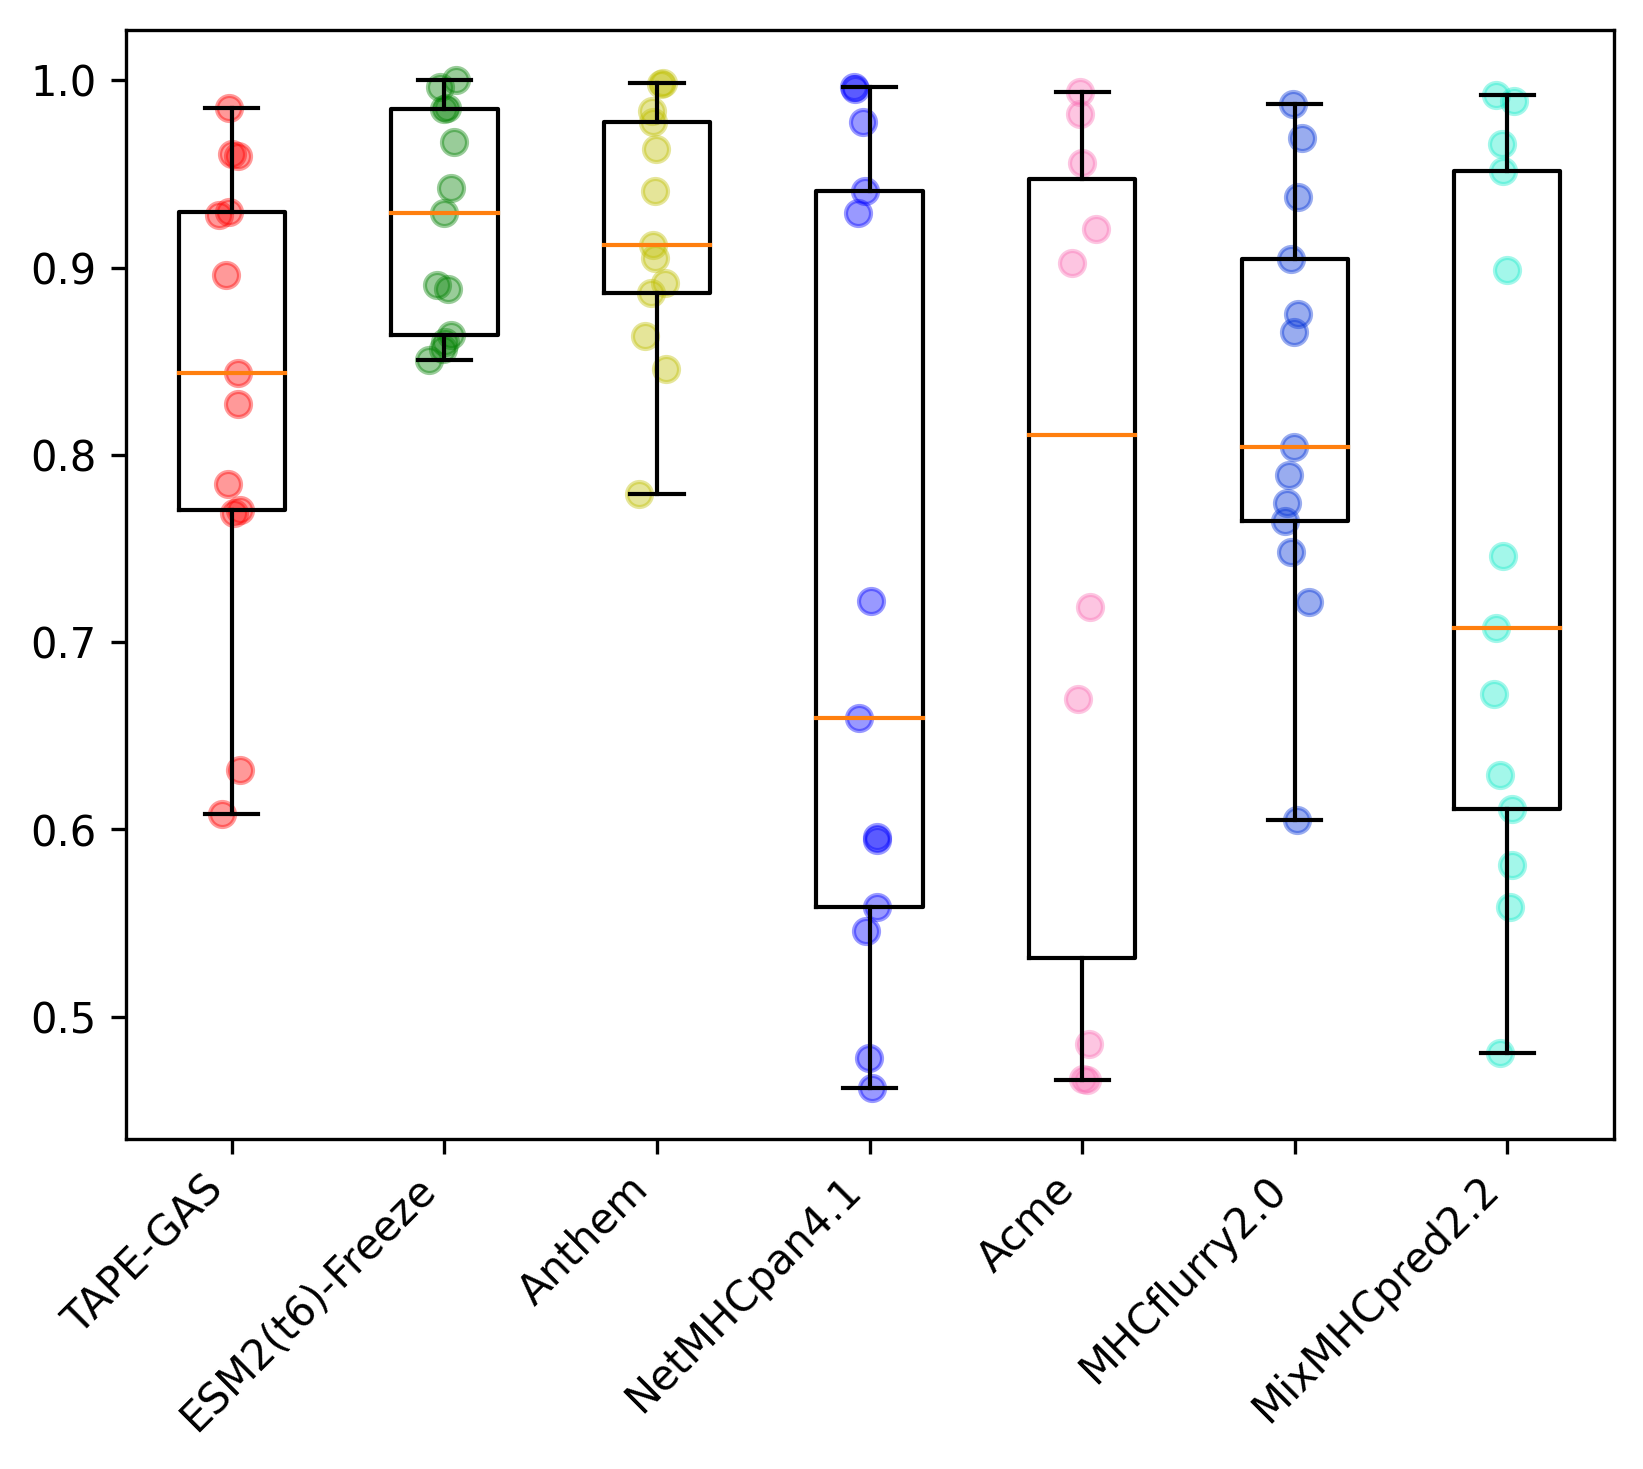
\includegraphics[width=\textwidth]{../img/results/auc_distribution_14-mer}
		\caption{14-mer}
		\label{fig:comparison_14}
	\end{subfigure}
	\caption{The AUC distribution for TAPE-GAS and ESM2(t6)-Freeze, both trained for 30 epochs, along with Anthem, NetMHCpan4.1, ACME, MixMHCpred2.2, and MHCflurry2.0.}
	\label{fig:auc_distribution}
\end{figure*}
